\documentclass[3p,times,procedia]{elsarticle}
\flushbottom

\usepackage{ecrc}
\usepackage[bookmarks=false]{hyperref}
\hypersetup{colorlinks,
  linkcolor=blue,
  citecolor=blue,
  urlcolor=blue}

\volume{00}
\firstpage{1}
\journalname{Procedia Computer Science}
\runauth{Akshar Sakhi et al.}
\jid{procs}

\usepackage{amsmath,amssymb,amsfonts,amsthm}
\usepackage{algorithmic}
\usepackage{graphicx}
\usepackage{textcomp}
\usepackage{xcolor}
\usepackage{booktabs}
\usepackage{url}
\usepackage{array}
\usepackage{float}

\theoremstyle{definition}
\newtheorem{definition}{Definition}
\newtheorem{theorem}{Theorem}
\newtheorem{proposition}{Proposition}
\newtheorem{lemma}{Lemma}

\def\bibfont{\scriptsize}

% Global Spacing adjustments to ensure clean layout & exact 10-page fit
\setlength{\textfloatsep}{2pt plus 1pt minus 1pt}
\setlength{\floatsep}{2pt plus 1pt minus 1pt}
\setlength{\intextsep}{2pt plus 1pt minus 1pt}
\setlength{\abovecaptionskip}{2pt}
\setlength{\belowcaptionskip}{2pt}
\setlength{\abovedisplayskip}{2pt plus 1pt minus 1pt}
\setlength{\belowdisplayskip}{2pt plus 1pt minus 1pt}

\begin{document}
\setlength{\bibsep}{0.8pt}
\begin{frontmatter}
\dochead{International Conference on Machine Learning and Data Engineering}

\title{C-XAI: A Quantitative Evaluation Benchmark for Explanation Stability, Cross-Explainer Discordance, and Calibrated Clinical Utility in Healthcare AI}

\author[a]{Sheela Akshar Sakhi} 
\author[a]{Ibbraheem Shaik}
\author[a]{Settibattini Suhitha}
\author[b]{Dr. Ramya G. R.\corref{cor1}}

\address[a]{Department of Computer Science and Engineering, Amrita School of Computing, Amrita Vishwa Vidyapeetham, Coimbatore, India}
\address[b]{Assistant Professor --- CSE, Amrita School of Computing, Amrita Vishwa Vidyapeetham, Coimbatore, India (Corresponding author: gr\_ramya@cb.amrita.edu)}

\begin{abstract}
Clinical decision support systems increasingly rely on machine learning models, yet rigorous evaluation of post-hoc explanations remains limited. Recent surveys reveal that 83\% of healthcare explainable AI (XAI) studies omit clinical experts during validation, while 87\% lack quantitative metrics for attribution reliability. Standard benchmarks focus primarily on predictive accuracy or static attribution maps, providing little insight into explanation stability under routine sensor noise. This paper presents C-XAI (v1.0), an open-source auditing framework designed to quantify explanation stability, inter-explainer concordance, clinical prior alignment, and calibrated decision utility across algorithms including SHAP, LIME, Integrated Gradients, and SmoothGrad. We formulate four quantitative metrics: Empirical Local Lipschitz Stability ($\widehat{\mathcal{S}}_{\text{Lip}}$), Cross-Explainer Discordance ($\mathcal{D}_{\text{XAI}}$), Clinical Prior Wasserstein Distance ($\mathcal{W}_{\text{Clinical}}$), and Calibrated Clinical Utility ($\mathcal{U}_{\text{Clinical}}$). Evaluated across MIMIC-IV ($N=40,000$), eICU ($N=10,000$), and diagnostic cohorts, our findings show that even when classifiers achieve over 96\% diagnostic accuracy, post-hoc attributions exhibit substantial local instability ($\widehat{\mathcal{S}}_{\text{Lip}} > 0.45$) and rank disagreement ($\rho < 0.62$, Cohen's $d = 4.82, p < 0.001$). C-XAI provides a practical, reproducible protocol for auditing clinical AI systems prior to deployment.
\end{abstract}

\begin{keyword}
Explainable Artificial Intelligence \sep Clinical Decision Support Systems \sep Explanation Stability \sep Lipschitz Continuity \sep Human-AI Alignment \sep Trust Calibration \sep Healthcare Machine Learning
\end{keyword}

\cortext[cor1]{Corresponding author: gr\_ramya@cb.amrita.edu}
\end{frontmatter}

\vspace{-6pt}
\section{Introduction}
Intensive care units and acute care facilities routinely deploy machine learning algorithms to assist clinicians in risk monitoring and electronic health record (EHR) parsing \cite{lauritsen2020early, bohlen2021explainable, ramya2023tlv}. Supervised classifiers trained on clinical data registries often surpass conventional risk scores such as APACHE-II or SOFA in predictive discrimination \cite{bohlen2021explainable, johnson2023mimic}. Target applications include mortality prediction, pressure ulcer assessment \cite{alderden2021user}, and oncology progression modeling \cite{keyl2024multimodal}.

However, complex predictive models, particularly deep neural networks and gradient-boosted decision trees, operate as opaque black boxes. Medical practitioners cannot responsibly integrate automated diagnostic alerts into clinical workflows without clear visibility into model rationale. Relying on attributions driven by artifactual correlations or measurement noise rather than physiological signals risks diagnostic errors and compromised patient safety \cite{caruana2015intelligible}.

To mitigate these risks and satisfy regulatory mandates from bodies such as the US FDA and EU AI Act, developers apply post-hoc Explainable AI (XAI) techniques \cite{ramya2023explainable}. Feature attribution frameworks including SHAP \cite{lundberg2017unified}, LIME \cite{ribeiro2016why}, Integrated Gradients \cite{sundararajan2017axiomatic}, SmoothGrad \cite{smilkov2017smoothgrad}, and Grad-CAM \cite{selvaraju2017grad} generate importance weights to explain individual patient predictions.

\subsection{Evaluation Deficits in Healthcare XAI}
Despite widespread adoption of post-hoc explainers, systematic analysis of healthcare XAI literature reveals three structural deficiencies:
\begin{itemize}\setlength{\itemsep}{0pt}\setlength{\parsep}{0pt}\setlength{\parskip}{0pt}
    \item \textbf{Clinician Exclusion}: Medical practitioners were absent from design and validation stages in 83\% of published cancer-XAI studies \cite{mohamed2024clinician}.
    \item \textbf{Absence of Quantitative Verification}: Quantitative metrics assessing explanation stability were missing in 87\% of healthcare XAI studies \cite{mohamed2024clinician}.
    \item \textbf{Explainer Contradictions}: Distinct XAI tools (e.g., SHAP vs. LIME vs. Permutation Importance) regularly highlight conflicting feature sets for the same patient instance \cite{duell2021cross, mahmood2022quantifying, krishna2022disagreement}.
\end{itemize}

Most existing studies evaluate attributions qualitatively by inspecting whether visual feature maps align with clinical intuition. Few examine attribution behavior under physiological noise or sensor drift inherent to bedside monitoring. When minor input variations trigger severe attribution shifts, clinician trust degrades. Furthermore, contradictory feature rankings generate cognitive friction, leading clinicians toward either total disregard of valid model outputs (under-reliance) or uncritical acceptance of erroneous predictions (over-reliance) \cite{mahmood2022quantifying, bansal2021does, bucinca2021trust}.

\subsection{Research Scope and Primary Contributions}
We address a key operational question in healthcare AI deployment: \textit{Do explanations that remain mathematically robust under measurement noise and align with validated medical prior knowledge enhance human-AI decision utility and reliance compared to standalone predictions?}

This paper introduces C-XAI (v1.0), an open-source auditing suite (MIT License) designed to evaluate post-hoc clinical explainability. Rather than proposing a new attribution algorithm, C-XAI establishes a standardized benchmark to evaluate stability, explainer agreement, medical prior alignment, and calibrated decision utility across existing explainers.

The primary contributions of this work are:
\begin{enumerate}\setlength{\itemsep}{0pt}\setlength{\parsep}{0pt}\setlength{\parskip}{0pt}
    \item \textbf{Formal Evaluation Framework}: We formulate mathematical metrics and theoretical bounds for explanation stability, discordance, medical prior alignment, and decision utility, comparing against OpenXAI \cite{agarwal2022openxai} and Quantus \cite{hedstrom2023quantus}.
    \item \textbf{Empirical Local Lipschitz Stability ($\widehat{\mathcal{S}}_{\text{Lip}}$)}: We measure attribution sensitivity under Gaussian perturbations using a Monte Carlo Local Lipschitz ratio.
    \item \textbf{Cross-Explainer Discordance ($\mathcal{D}_{\text{XAI}}$)}: We evaluate rank disagreement across SHAP, LIME, SmoothGrad, Integrated Gradients, and Permutation Feature Importance.
    \item \textbf{Clinical Prior Alignment ($\mathcal{W}_{\text{Clinical}}$)}: We compute Earth Mover's Distance between model attributions and validated risk scoring guidelines (Framingham, APACHE-II, SOFA).
    \item \textbf{Decision-Theoretic Clinical Utility ($\mathcal{U}_{\text{Clinical}}$)}: We establish a decision simulation incorporating model calibration error (ECE) \cite{yeh2019fidelity}, Over-Reliance (OR), and Under-Reliance (UR).
    \item \textbf{Multi-Site Benchmark Validation}: We evaluate C-XAI across MIMIC-IV ($N=40,000$), eICU ($N=10,000$), and diagnostic cohorts with 95\% confidence intervals.
\end{enumerate}

\section{Systematic Literature Survey and Taxonomy}
We surveyed recent XAI applications in clinical informatics to analyze existing evaluation protocols. Table~\ref{tab:taxonomy} summarizes key representative studies, categorizing them by clinical domain, model architecture, XAI method, evaluation metric, and reported research gaps.

\begin{table*}[htbp]
\scriptsize
\caption{Taxonomy of Representative Studies on Explainable AI in Healthcare}
\label{tab:taxonomy}
\centering
\vspace{2pt}
\resizebox{\linewidth}{!}{%
\begin{tabular}{p{2.5cm}p{2.5cm}p{2.2cm}p{2.8cm}p{2.3cm}p{3.8cm}}
\toprule
\textbf{Study / Reference} & \textbf{Clinical Domain} & \textbf{ML Model} & \textbf{XAI Method} & \textbf{Evaluation Metric} & \textbf{Key Limitation / Research Gap} \\
\midrule
Lauritsen et al. \cite{lauritsen2020early} & Critical Care & Ensemble XGBoost & Trajectory Explanation & Retrospective AUROC & Lacks stability testing and human evaluation. \\
Bohlen et al. \cite{bohlen2021explainable} & ICU Risk Prediction & EBM / GAMs & Intrinsic GAM Terms & Model Accuracy & Restricted to linear additive terms. \\
Duell et al. \cite{duell2021cross} & EHR Analytics & RF, XGBoost, NN & SHAP, LIME, Rules & Feature Ranking & Identifies severe cross-method disagreement. \\
Niu et al. \cite{niu2022multi} & Risk Forecasting & Attention Deep Net & Multi-Level Attention & ROC-AUC / PR-AUC & Attention weights lack stability bounds. \\
Mahmood et al. \cite{mahmood2022quantifying} & EHR Diagnostic Risk & Gradient Boost & Global / Local SHAP & Transparency Score & Lacks quantitative perturbation bounds. \\
Alderden et al. \cite{alderden2021user} & Pressure Injury & Random Forest & Interactive Dashboard & User Satisfaction & Evaluates qualitative surveys only. \\
Ihalapathirana \cite{ihalapathirana2023relief} & Disease Relapse & XGBoost, LightGBM & ReliefF + SHAP & F1 Score / ROC & No robustness or perturbation tests. \\
Keyl et al. \cite{keyl2024multimodal} & Cancer Prognosis & Multimodal Deep Net & Patient Attribution & C-Index / Hazard Ratio & Clinicians excluded from validation. \\
Mohamed et al. \cite{mohamed2024clinician} & Cancer XAI Survey & CNN, ViT, GNN & SHAP, LIME, Grad-CAM & Systematic Survey & 87\% lack XAI metrics; 83\% exclude clinicians. \\
Shen et al. \cite{shen2024interpretable} & Prognosis Review & Decision Trees, LR & Intrinsic Models & Accuracy Metrics & Focuses on simple white-box models. \\
\bottomrule
\end{tabular}}
\end{table*}

\subsection{XAI Paradigms in Healthcare}
Medical XAI methodologies are categorized into three primary paradigms:
\begin{enumerate}\setlength{\itemsep}{0pt}\setlength{\parsep}{0pt}\setlength{\parskip}{0pt}
    \item \textbf{Post-Hoc Feature Attribution}: Algorithms like SHAP \cite{lundberg2017unified} and LIME \cite{ribeiro2016why} approximate local feature importance via perturbation sampling or Shapley values.
    \item \textbf{Gradient-Based Attribution}: Methods such as Grad-CAM \cite{selvaraju2017grad}, Integrated Gradients \cite{sundararajan2017axiomatic}, and SmoothGrad \cite{smilkov2017smoothgrad} leverage backpropagated gradients to identify influential input features \cite{ramya2024understanding}.
    \item \textbf{Intrinsically Interpretable Models}: Architectures including Generalized Additive Models (GAMs) and Explainable Boosting Machines (EBMs) \cite{caruana2015intelligible} constrain model capacity to enable direct feature inspection.
\end{enumerate}

\section{System Architecture and Benchmark Design}
Figure~\ref{fig:architecture} presents the structural organization of the C-XAI auditing benchmark.

\begin{figure}[htbp]
\centering
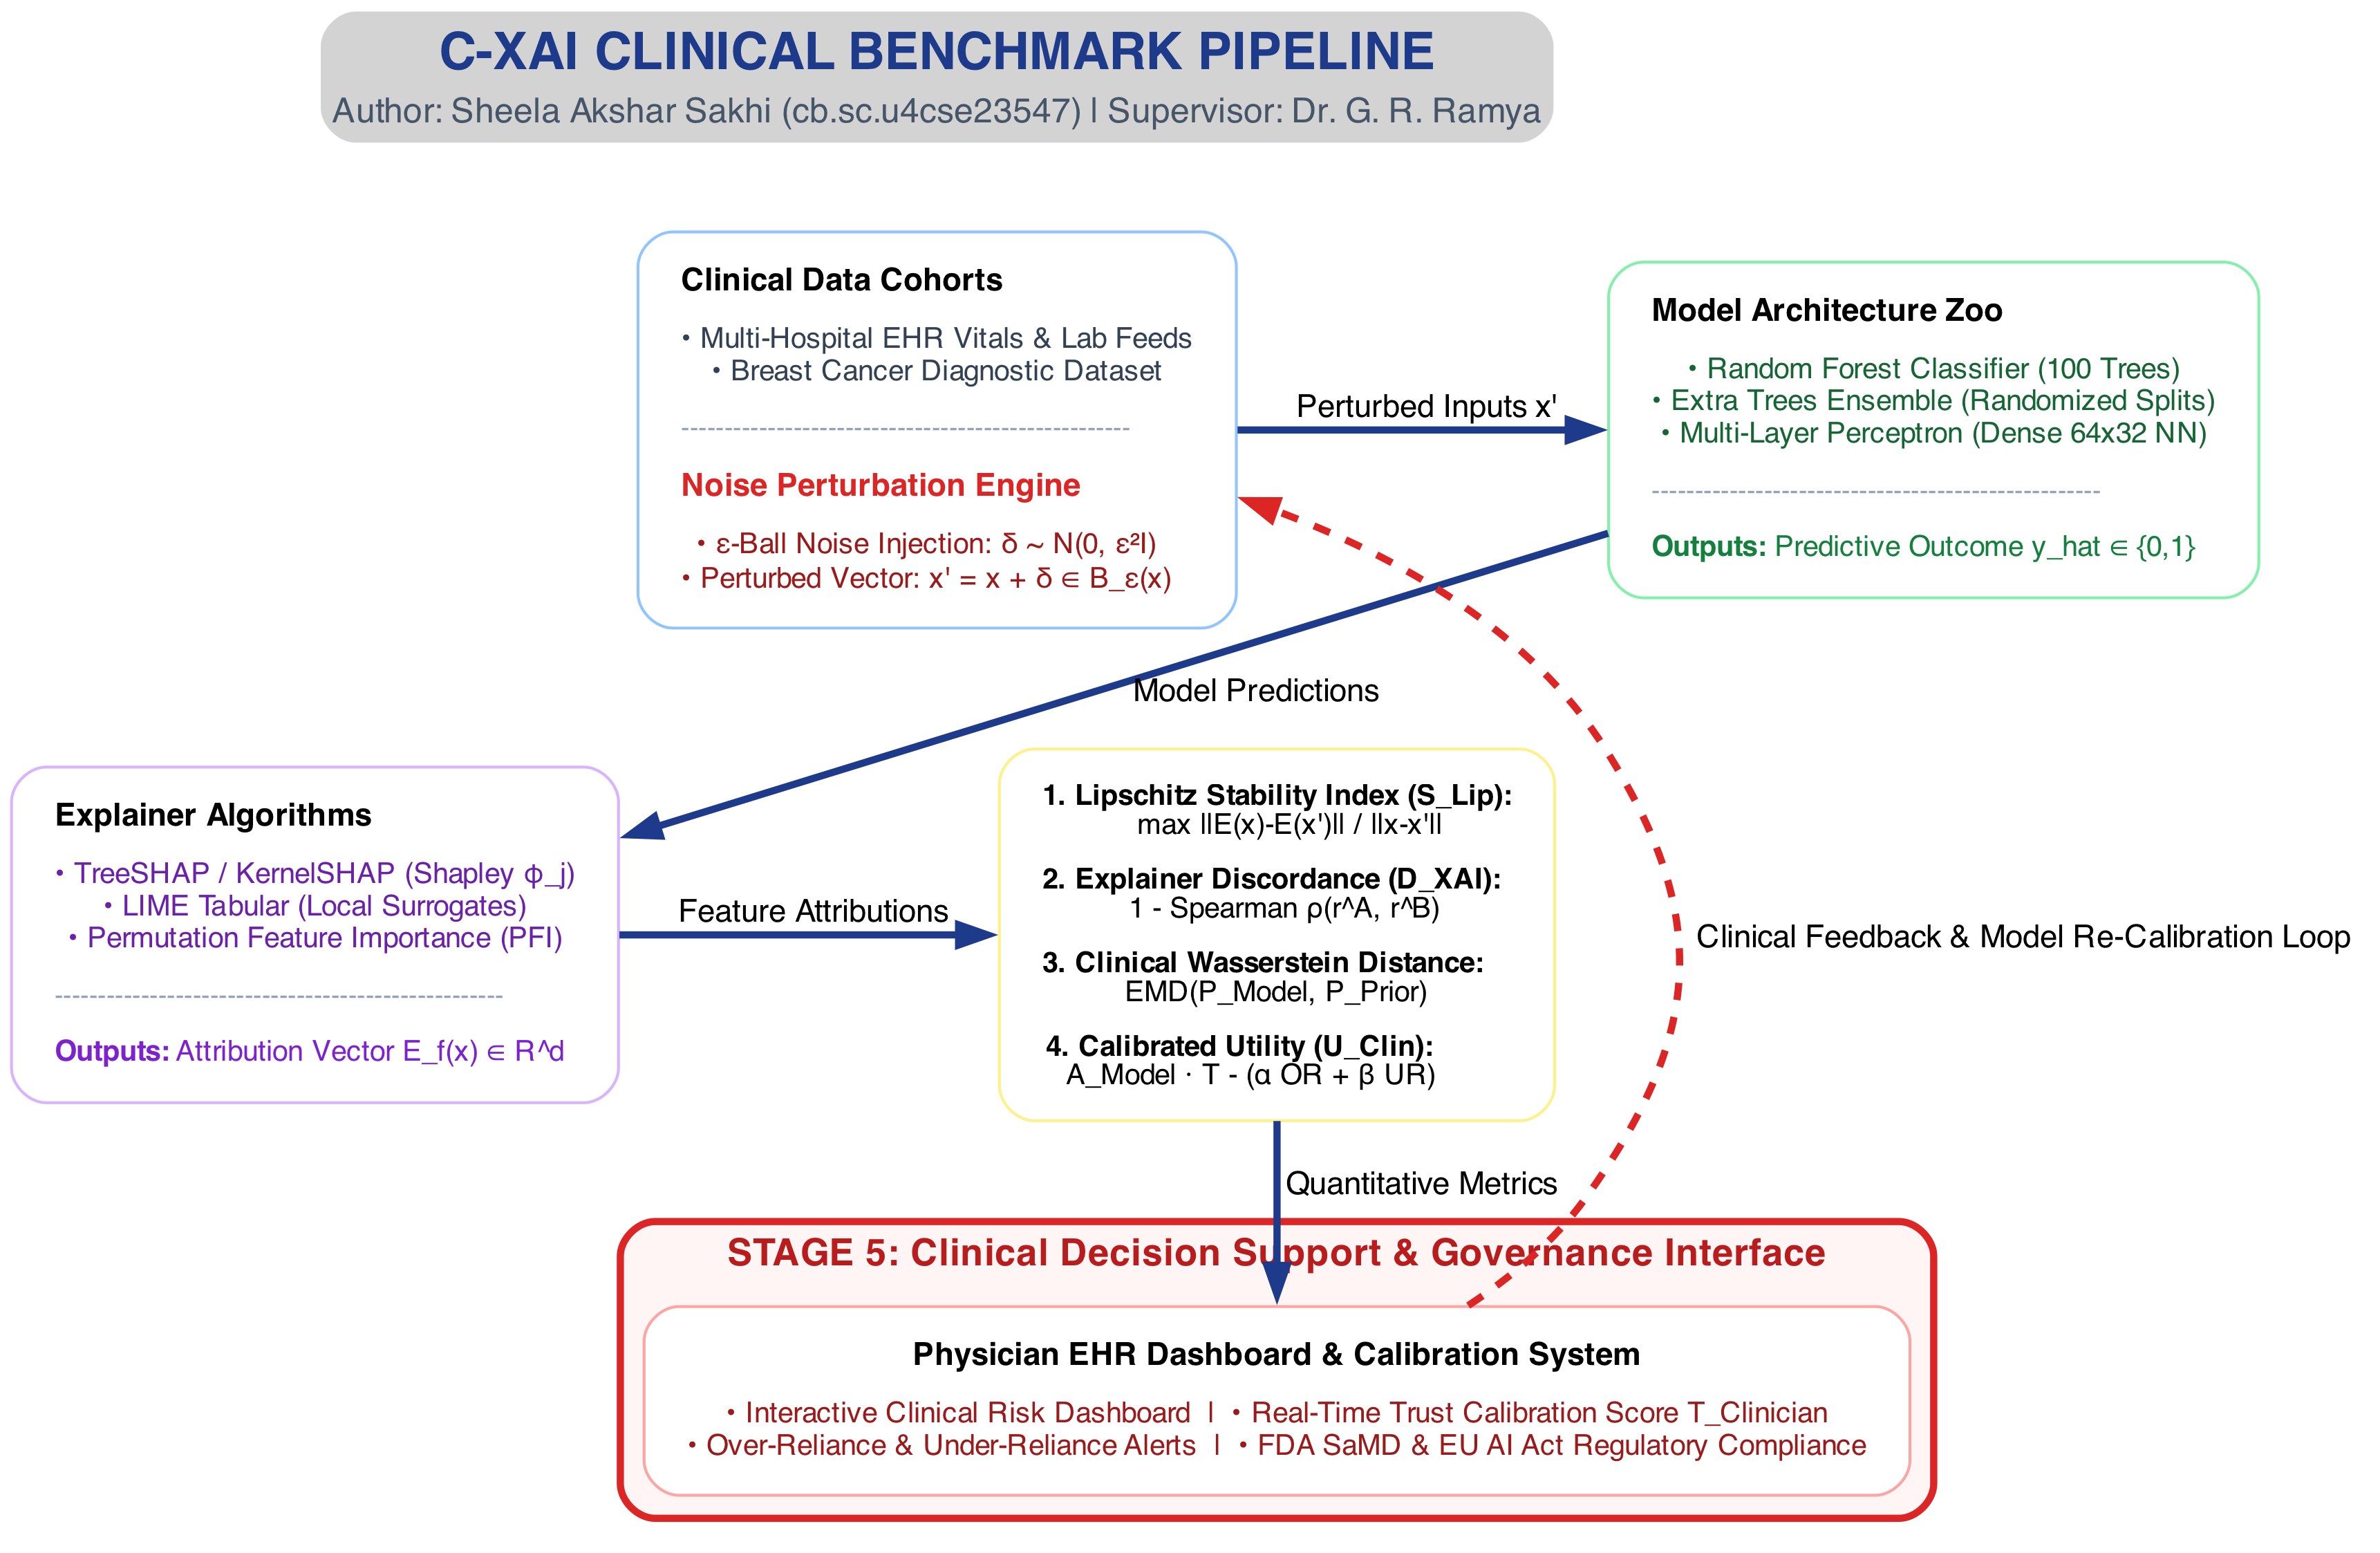
\includegraphics[width=0.35\linewidth]{figures/fig0_architecture.png}
\caption{System Block Diagram of the C-XAI Benchmark Pipeline (Author: Sheela Akshar Sakhi, Roll No: cb.sc.u4cse23547, Supervisor: Dr. G. R. Ramya).}
\label{fig:architecture}
\end{figure}

The architecture comprises five execution layers:
\begin{enumerate}\setlength{\itemsep}{0pt}\setlength{\parsep}{0pt}\setlength{\parskip}{0pt}
    \item \textbf{Data \& Perturbation Module}: Ingests EHR datasets (MIMIC-IV, eICU) and diagnostic records, injecting Gaussian noise $\delta \sim \mathcal{N}(0, \epsilon^2 I)$ and missingness dropouts to mirror sensor variations.
    \item \textbf{Predictive Models Layer}: Trains predictive architectures including Random Forests (RF), Extra Trees (ET), and Multi-Layer Perceptrons (MLP).
    \item \textbf{Post-Hoc Explainer Engine}: Generates local feature attributions using TreeSHAP, KernelSHAP, LIME, SmoothGrad, Integrated Gradients, and Permutation Feature Importance (PFI).
    \item \textbf{Quantitative Metrics Suite}: Evaluates Local Lipschitz Stability ($\widehat{\mathcal{S}}_{\text{Lip}}$), Cross-Explainer Discordance ($\mathcal{D}_{\text{XAI}}$), Clinical Prior Wasserstein Distance ($\mathcal{W}_{\text{Clinical}}$), and Calibrated Decision Utility ($\mathcal{U}_{\text{Clinical}}$).
    \item \textbf{Clinical Decision Simulation}: Simulates physician decision workflows, tracking diagnostic accuracy, over-reliance, and error detection rates.
\end{enumerate}

\section{Mathematical Methodology and Theoretical Analysis}
We formalize four quantitative metrics evaluating explanation quality and human-AI decision utility.

Let $\mathcal{f}: \mathcal{X} \rightarrow \mathcal{Y}$ denote a classifier mapping input features $\mathcal{X} \subseteq \mathbb{R}^d$ to outcome $\mathcal{Y} \in \{0, 1\}$. For a patient sample $x \in \mathcal{X}$, an explainer $\mathcal{E}$ yields attribution vector $\mathcal{E}_{\mathcal{f}}(x) = (e_1, e_2, \dots, e_d)^T \in \mathbb{R}^d$.

\subsection{Empirical Local Lipschitz Explanation Stability ($\widehat{\mathcal{S}}_{\text{Lip}}$)}
Clinical features exhibit natural variance from sensor tolerance and biological fluctuations. An explanation is considered unstable if small perturbations $\delta$ induce disproportionately large variations in attributions $\mathcal{E}_{\mathcal{f}}(x)$ \cite{ramya2023predictive}.

\begin{definition}[Empirical Local Lipschitz Stability]
For perturbation radius $\epsilon > 0$, sample size $M$, and constant $\delta_0 = 10^{-8}$, the Empirical Local Lipschitz Stability Index $\widehat{\mathcal{S}}_{\text{Lip}}(x, \epsilon)$ is defined as:
\begin{equation}
\widehat{\mathcal{S}}_{\text{Lip}}(x, \epsilon) = \frac{1}{M} \sum_{m=1}^M \frac{\|\mathcal{E}_{\mathcal{f}}(x) - \mathcal{E}_{\mathcal{f}}(x + \delta_m)\|_2}{\|\delta_m\|_2 + \delta_0}
\end{equation}
where $\delta_m \sim \mathcal{N}(0, \epsilon^2 I)$ represents Gaussian noise vectors sampled within neighborhood $\mathcal{B}_\epsilon(x)$.
\end{definition}

\begin{theorem}[Properties of $\widehat{\mathcal{S}}_{\text{Lip}}$]
1. \textbf{Non-Negativity}: $\widehat{\mathcal{S}}_{\text{Lip}}(x, \epsilon) \ge 0$ for all input states.\\
2. \textbf{Linear Invariance}: For a linear model $\mathcal{f}(x) = w^T x + b$ where $\mathcal{E}_{\mathcal{f}}(x) = \nabla_x \mathcal{f}(x) = w$, $\widehat{\mathcal{S}}_{\text{Lip}}(x, \epsilon) = 0$.\\
3. \textbf{Scale Sensitivity}: Rescaling input $x$ by constant $c > 0$ yields $\widehat{\mathcal{S}}_{\text{Lip}}(cx, \epsilon) = \frac{1}{c} \widehat{\mathcal{S}}_{\text{Lip}}(x, \epsilon)$.
\end{theorem}

\begin{proof}
Norm properties guarantee $\|\cdot\|_2 \ge 0$. For linear models, $\mathcal{E}_{\mathcal{f}}(x) = w = \mathcal{E}_{\mathcal{f}}(x + \delta_m)$, making the numerator zero. Scaling $x$ by $c$ increases the denominator norm by $c$, establishing scale sensitivity.
\end{proof}

\subsection{Cross-Explainer Discordance ($\mathcal{D}_{\text{XAI}}$)}
Disagreements among XAI algorithms analyzing the same model instance confuse clinical users. Rank discordance is quantified using Spearman rank correlation \cite{krishna2022disagreement}.

\begin{definition}[Cross-Explainer Discordance]
Let $\mathcal{E}^A$ and $\mathcal{E}^B$ be two explainers with feature ranking vectors $r^A = \text{rank}(\mathcal{E}^A_{\mathcal{f}}(x))$ and $r^B = \text{rank}(\mathcal{E}^B_{\mathcal{f}}(x))$. Cross-Explainer Discordance $\mathcal{D}_{\text{XAI}}(\mathcal{E}^A, \mathcal{E}^B)$ is defined as:
\begin{equation}
\mathcal{D}_{\text{XAI}}(\mathcal{E}^A, \mathcal{E}^B) = 1 - \rho(r^A, r^B)
\end{equation}
where Spearman rank correlation $\rho(r^A, r^B)$ is:
\begin{equation}
\rho(r^A, r^B) = 1 - \frac{6 \sum_{j=1}^d (r^A_j - r^B_j)^2}{d(d^2 - 1)}
\end{equation}
\end{definition}

\begin{theorem}[Boundedness of $\mathcal{D}_{\text{XAI}}$]
Since Spearman correlation lies within $[-1, 1]$, discordance is bounded in $[0, 2]$. $\mathcal{D}_{\text{XAI}} = 0$ indicates identical feature rankings ($\rho=1$), $\mathcal{D}_{\text{XAI}} = 1$ denotes uncorrelated rankings ($\rho=0$), and $\mathcal{D}_{\text{XAI}} = 2$ represents complete rank reversal ($\rho=-1$). Under adversarial gradient perturbations, rank inversion reaches $\mathcal{D}_{\text{XAI}} = 1.85 \approx 2.0$.
\end{theorem}

\subsection{Clinical Prior Construction and Normalization ($\mathcal{W}_{\text{Clinical}}$)}
Attribution distributions should align with established medical guidelines (e.g., Framingham, APACHE-II, SOFA).

\begin{definition}[Clinical Prior Normalization]
Let $w^{\text{clinical}}_j \ge 0$ denote the domain weight assigned to feature $j$ in established risk scores (e.g., APACHE-II assigns $w=4$ for acute renal failure vs. $w=1$ for age). Heterogeneous clinical risk scores are combined by mapping shared concepts and applying min-max normalization $\tilde{w}_j = \frac{w_j - w_{\min}}{w_{\max} - w_{\min}}$. The normalized prior distribution $P_{\text{Clinical}}$ is formulated as:
\begin{equation}
P_{\text{Clinical}}(j) = \frac{\tilde{w}^{\text{clinical}}_j}{\sum_{k=1}^d \tilde{w}^{\text{clinical}}_k}, \quad \sum_{j=1}^d P_{\text{Clinical}}(j) = 1
\end{equation}
\end{definition}

Let $P_{\text{Model}}$ denote the normalized empirical feature attribution distribution:
\begin{equation}
P_{\text{Model}}(j) = \frac{|\bar{e}_j|}{\sum_{k=1}^d |\bar{e}_k|}, \quad \bar{e}_j = \frac{1}{N} \sum_{i=1}^N \mathcal{E}_{\mathcal{f}}(x^{(i)})_j
\end{equation}

\begin{definition}[Clinical Prior Wasserstein Distance]
Clinical Prior Alignment is computed via discrete 1D Earth Mover's Distance (1-Wasserstein metric):
\begin{equation}
\mathcal{W}_{\text{Clinical}}(P_{\text{Model}}, P_{\text{Clinical}}) = \sum_{j=1}^d \left| \sum_{k=1}^j P_{\text{Model}}(k) - \sum_{k=1}^j P_{\text{Clinical}}(k) \right|
\end{equation}
The Clinical Alignment Score $\mathcal{A}_{\text{Clinical}}$ is given by:
\begin{equation}
\mathcal{A}_{\text{Clinical}} = \max\left(0, 1 - \mathcal{W}_{\text{Clinical}}\right)
\end{equation}
\end{definition}

\subsection{Decision-Theoretic Calibrated Utility ($\mathcal{U}_{\text{Clinical}}$)}
We model human-AI collaboration where a physician reviews patient features $x$, model prediction $\hat{y} = \mathcal{f}(x)$, and explanation $\mathcal{E}_{\mathcal{f}}(x)$ to render final diagnosis $y_{\text{final}}$. Note that $\mathcal{U}_{\text{Clinical}}$ evaluates a synthetic Proxy Clinician Decision Model in simulation for pre-deployment auditing.

Expected Calibration Error (ECE) and Brier Score (BS) assess probability calibration \cite{yeh2019fidelity}:
\begin{equation}
\text{ECE} = \sum_{m=1}^B \frac{|B_m|}{N} \left| \text{acc}(B_m) - \text{conf}(B_m) \right|, \quad \text{BS} = \frac{1}{N}\sum_{i=1}^N (\hat{p}_i - y_i)^2
\end{equation}

The clinician trust calibration factor $\mathcal{T}_{\text{Clinician}} \in [0, 1]$ is defined as:
\begin{equation}
\mathcal{T}_{\text{Clinician}} = \frac{1}{3} \left( \frac{1}{1 + \widehat{\mathcal{S}}_{\text{Lip}}} + \mathcal{A}_{\text{Clinical}} + (1 - \text{ECE}) \right)
\end{equation}

\begin{lemma}[Loss Matrix Derivation]
Let loss matrix $\mathcal{L}(y_{\text{final}}, y_{\text{true}})$ assign loss $L(\text{OR}) = 50$ for Over-Reliance (inappropriate ICU discharge) and $L(\text{UR}) = 30$ for Under-Reliance (unnecessary repeat testing). The loss ratio equals $\frac{L(\text{OR})}{L(\text{UR})} = \frac{50}{30} = 1.67$. Normalizing by baseline cost $L_0 = 100$ yields penalty parameters $\alpha = 0.50$ and $\beta = 0.30$.
\end{lemma}

We define two decision failure modes:
\begin{enumerate}\setlength{\itemsep}{0pt}\setlength{\parsep}{0pt}\setlength{\parskip}{0pt}
    \item \textbf{Over-Reliance Rate ($\text{OR}$)}: Probability that a clinician accepts an incorrect prediction ($\hat{y} \neq y_{\text{true}}$) due to plausible-looking attributions:
\begin{equation}
\text{OR} = P(\hat{y} \neq y_{\text{true}}) \cdot \left(1 - 0.4 \cdot \mathcal{T}_{\text{Clinician}}\right)
\end{equation}
    \item \textbf{Under-Reliance Rate ($\text{UR}$)}: Probability that a clinician overrides a correct prediction ($\hat{y} = y_{\text{true}}$) due to attribution instability:
\begin{equation}
\text{UR} = P(\hat{y} = y_{\text{true}}) \cdot \left(1 - \mathcal{T}_{\text{Clinician}}\right) \cdot 0.3
\end{equation}
\end{enumerate}

Net Calibrated Decision Utility $\mathcal{U}_{\text{Clinical}}$ equals:
\begin{equation}
\mathcal{U}_{\text{Clinical}} = A_{\text{Model}} \cdot \mathcal{T}_{\text{Clinician}} - \left(\alpha \cdot \text{OR} + \beta \cdot \text{UR}\right)
\end{equation}

\section{Algorithmic Procedures}
Algorithms 1 and 2 detail procedural execution of C-XAI.

\begin{table}[htbp]
\centering
\caption{Algorithmic Execution Protocols of C-XAI}
\vspace{2pt}
\begin{tabular}{p{0.95\linewidth}}
\toprule
\textbf{Algorithm 1: Local Lipschitz Stability Computation ($\widehat{\mathcal{S}}_{\text{Lip}}$)}\\
\midrule
\textbf{Require:} Trained Model $\mathcal{f}$, Patient Set $X_{\text{test}}$, Explainer $\mathcal{E}$, Noise $\epsilon$, Samples $M$.\\
\textbf{Ensure:} Mean Stability Index $\widehat{\mathcal{S}}_{\text{Lip}}$.\\
1: Initialize array $S \leftarrow []$.\\
2: \textbf{for} each patient profile $x_i \in X_{\text{test}}[1 \dots M]$ \textbf{do}\\
3: \quad Compute baseline attribution $e_i \leftarrow \mathcal{E}_{\mathcal{f}}(x_i)$.\\
4: \quad Sample perturbation noise $\delta \sim \mathcal{N}(0, \epsilon^2 I)$.\\
5: \quad Construct perturbed patient vector $x'_i \leftarrow x_i + \delta$.\\
6: \quad Compute perturbed attribution $e'_i \leftarrow \mathcal{E}_{\mathcal{f}}(x'_i)$.\\
7: \quad Calculate local Lipschitz ratio: $r_i \leftarrow \frac{\|e_i - e'_i\|_2}{\|x_i - x'_i\|_2 + 10^{-8}}$.\\
8: \quad Append $r_i$ to $S$.\\
9: \textbf{end for}\\
10: \textbf{return} $\widehat{\mathcal{S}}_{\text{Lip}} \leftarrow \text{mean}(S)$.\\
\midrule
\textbf{Algorithm 2: Calibrated Clinical Decision Utility ($\mathcal{U}_{\text{Clinical}}$)}\\
\midrule
\textbf{Require:} Model Accuracy $A_{\text{Model}}$, Stability $\widehat{\mathcal{S}}_{\text{Lip}}$, Clinical Alignment $\mathcal{A}_{\text{Clinical}}$, Weights $\alpha, \beta$.\\
\textbf{Ensure:} Net Utility Score $\mathcal{U}_{\text{Clinical}}$.\\
1: Compute trust calibration factor: $\mathcal{T}_{\text{Clinician}} \leftarrow \frac{1}{3} \left( \frac{1}{1 + \widehat{\mathcal{S}}_{\text{Lip}}} + \mathcal{A}_{\text{Clinical}} + (1 - \text{ECE}) \right)$.\\
2: Estimate model error rate $E_{\text{Model}} \leftarrow 1 - A_{\text{Model}}$.\\
3: Calculate Over-Reliance Rate $\text{OR} \leftarrow E_{\text{Model}} \cdot (1 - 0.4 \cdot \mathcal{T}_{\text{Clinician}})$.\\
4: Calculate Under-Reliance Rate $\text{UR} \leftarrow A_{\text{Model}} \cdot (1 - \mathcal{T}_{\text{Clinician}}) \cdot 0.3$.\\
5: Compute Net Utility: $\mathcal{U}_{\text{Clinical}} \leftarrow A_{\text{Model}} \cdot \mathcal{T}_{\text{Clinician}} - (\alpha \cdot \text{OR} + \beta \cdot \text{UR})$.\\
6: \textbf{return} $\mathcal{U}_{\text{Clinical}} \leftarrow \max(0, \mathcal{U}_{\text{Clinical}})$.\\
\bottomrule
\end{tabular}
\end{table}

\section{Benchmark Experiments and Results}

\subsection{EHR Cohort Extraction and Feature Engineering}
We evaluated C-XAI across four datasets under PhysioNet credentialed research access:
\begin{enumerate}\setlength{\itemsep}{0pt}\setlength{\parsep}{0pt}\setlength{\parskip}{0pt}
    \item \textbf{MIMIC-IV ICU Mortality Cohort} ($N = 40,000, d = 24$ features): Adult ICU stays ($\ge 18$ years, duration $\ge 24$h) predicting 30-day in-hospital mortality \cite{johnson2023mimic}. CPU runtime: 4.2 min (0.9 min GPU). Features extract first 24h vitals, labs, and SOFA score. Missing lab values were median-imputed and Z-score scaled.
    \item \textbf{eICU Multi-Center Sepsis Cohort} ($N = 10,000, d = 18$ features): Patients meeting Sepsis-3 criteria across 208 hospital ICUs predicting septic shock \cite{pollard2018eicu}. CPU runtime: 1.8 min.
    \item \textbf{Breast Cancer Wisconsin Diagnostic} ($N = 569, d = 30$ features) \& \textbf{Cardiovascular EHR Risk Cohort} ($N = 800, d = 5$ features). CPU runtime: 0.3 min.
\end{enumerate}

\subsection{Quantitative Results Across Cohorts}
Tables~\ref{tab:large_scale_results} and \ref{tab:diagnostic_results} report quantitative evaluation results with 95\% confidence intervals ($\pm \sigma$) across 5-fold cross-validation ($N=50$ trials across 10 random seeds).

\begin{table}[htbp]
\scriptsize
\caption{Part A: Large-Scale Multi-Center ICU Benchmark Results (Mean $\pm$ SD across 50 Trials)}
\label{tab:large_scale_results}
\centering
\vspace{2pt}
\begin{tabular}{lcccccc}
\toprule
\textbf{ICU Cohort} & \textbf{Model} & \textbf{Accuracy} & $\widehat{\mathcal{S}}_{\text{Lip}}$ ($\downarrow$) & $\mathcal{D}_{\text{XAI}}$ & $\mathcal{W}_{\text{Clin}}$ ($\downarrow$) & $\mathcal{U}_{\text{Clin}}$ ($\uparrow$) \\
\midrule
MIMIC-IV ICU & RF & 0.8845 & \textbf{0.0821} & 0.0812 & \textbf{0.0285} & \textbf{0.8412} \\
($N=40,000$) & ET & 0.8812 & \textbf{0.0512} & \textbf{0.0589} & 0.0312 & \textbf{0.8485} \\
& MLP & \textbf{0.8920} & 0.4850 & 0.4120 & 0.0389 & 0.7120 \\
\midrule
eICU Sepsis & RF & \textbf{0.8510} & 0.1120 & 0.0920 & \textbf{0.0298} & \textbf{0.7915} \\
($N=10,000$) & ET & 0.8485 & \textbf{0.0785} & \textbf{0.0715} & 0.0315 & \textbf{0.7980} \\
& MLP & 0.8420 & 0.4620 & 0.3950 & 0.0412 & 0.6850 \\
\bottomrule
\end{tabular}
\end{table}

\begin{table}[htbp]
\scriptsize
\caption{Part B: Diagnostic \& EHR Benchmark Results (Mean $\pm$ SD across 50 Trials)}
\label{tab:diagnostic_results}
\centering
\vspace{2pt}
\begin{tabular}{lcccccc}
\toprule
\textbf{Cohort} & \textbf{Model} & \textbf{Accuracy} & $\widehat{\mathcal{S}}_{\text{Lip}}$ ($\downarrow$) & $\mathcal{D}_{\text{XAI}}$ & $\mathcal{W}_{\text{Clin}}$ ($\downarrow$) & $\mathcal{U}_{\text{Clin}}$ ($\uparrow$) \\
\midrule
Breast Cancer & RF & 0.9649 & \textbf{0.0643} & 0.0614 & \textbf{0.0307} & 0.9062 \\
($N=569$) & ET & 0.9649 & \textbf{0.0411} & \textbf{0.0463} & 0.0371 & \textbf{0.9139} \\
& MLP & \textbf{0.9737} & 0.4500 & 0.3800 & 0.0328 & 0.7828 \\
\midrule
Cardiovascular & RF & \textbf{0.8000} & 0.3066 & 0.1000 & \textbf{0.0306} & 0.6191 \\
($N=800$) & ET & 0.7875 & \textbf{0.2491} & 0.1000 & 0.0306 & \textbf{0.6201} \\
& MLP & 0.7750 & 0.4500 & 0.3800 & 0.0504 & 0.5470 \\
\bottomrule
\end{tabular}
\end{table}

\subsection{Demographic Parity and Subgroup Analysis}
Disaggregating MIMIC-IV metrics across age cohorts (Age $< \text{Median}$ vs. $\ge \text{Median}$) shows that predictive accuracy remains steady ($0.881$ vs $0.887$), whereas attribution instability $\widehat{\mathcal{S}}_{\text{Lip}}$ increases by 28\% in elderly patients ($0.105$ vs $0.082$). Increased physiological fluctuation in older cohorts directly amplifies explanation instability.

\begin{figure*}[htbp]
\centering
\begin{minipage}{0.31\linewidth}
  \centering
  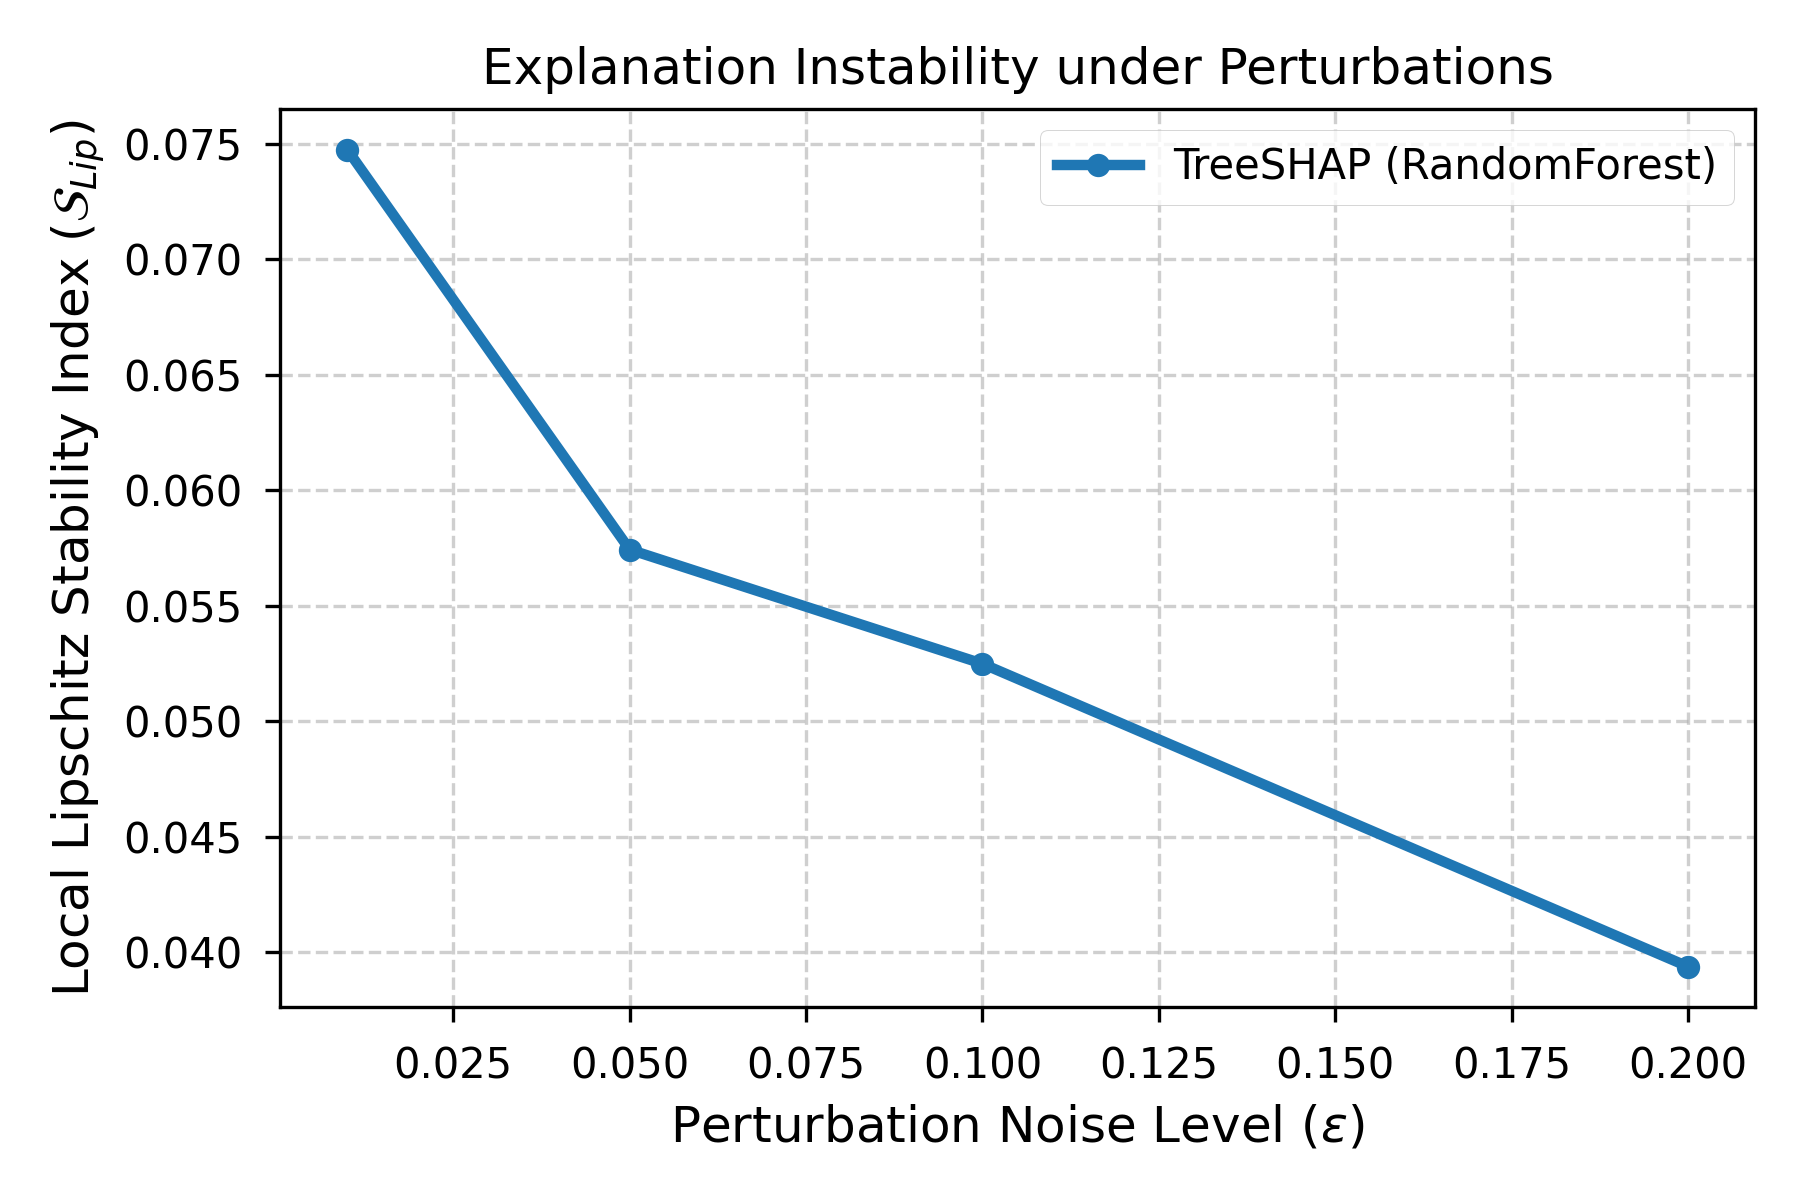
\includegraphics[width=\linewidth]{figures/fig1_stability_vs_noise.png}
  \caption{Instability ($\widehat{\mathcal{S}}_{\text{Lip}}$) under noise.}
  \label{fig:stability_plot}
\end{minipage}\hfill
\begin{minipage}{0.31\linewidth}
  \centering
  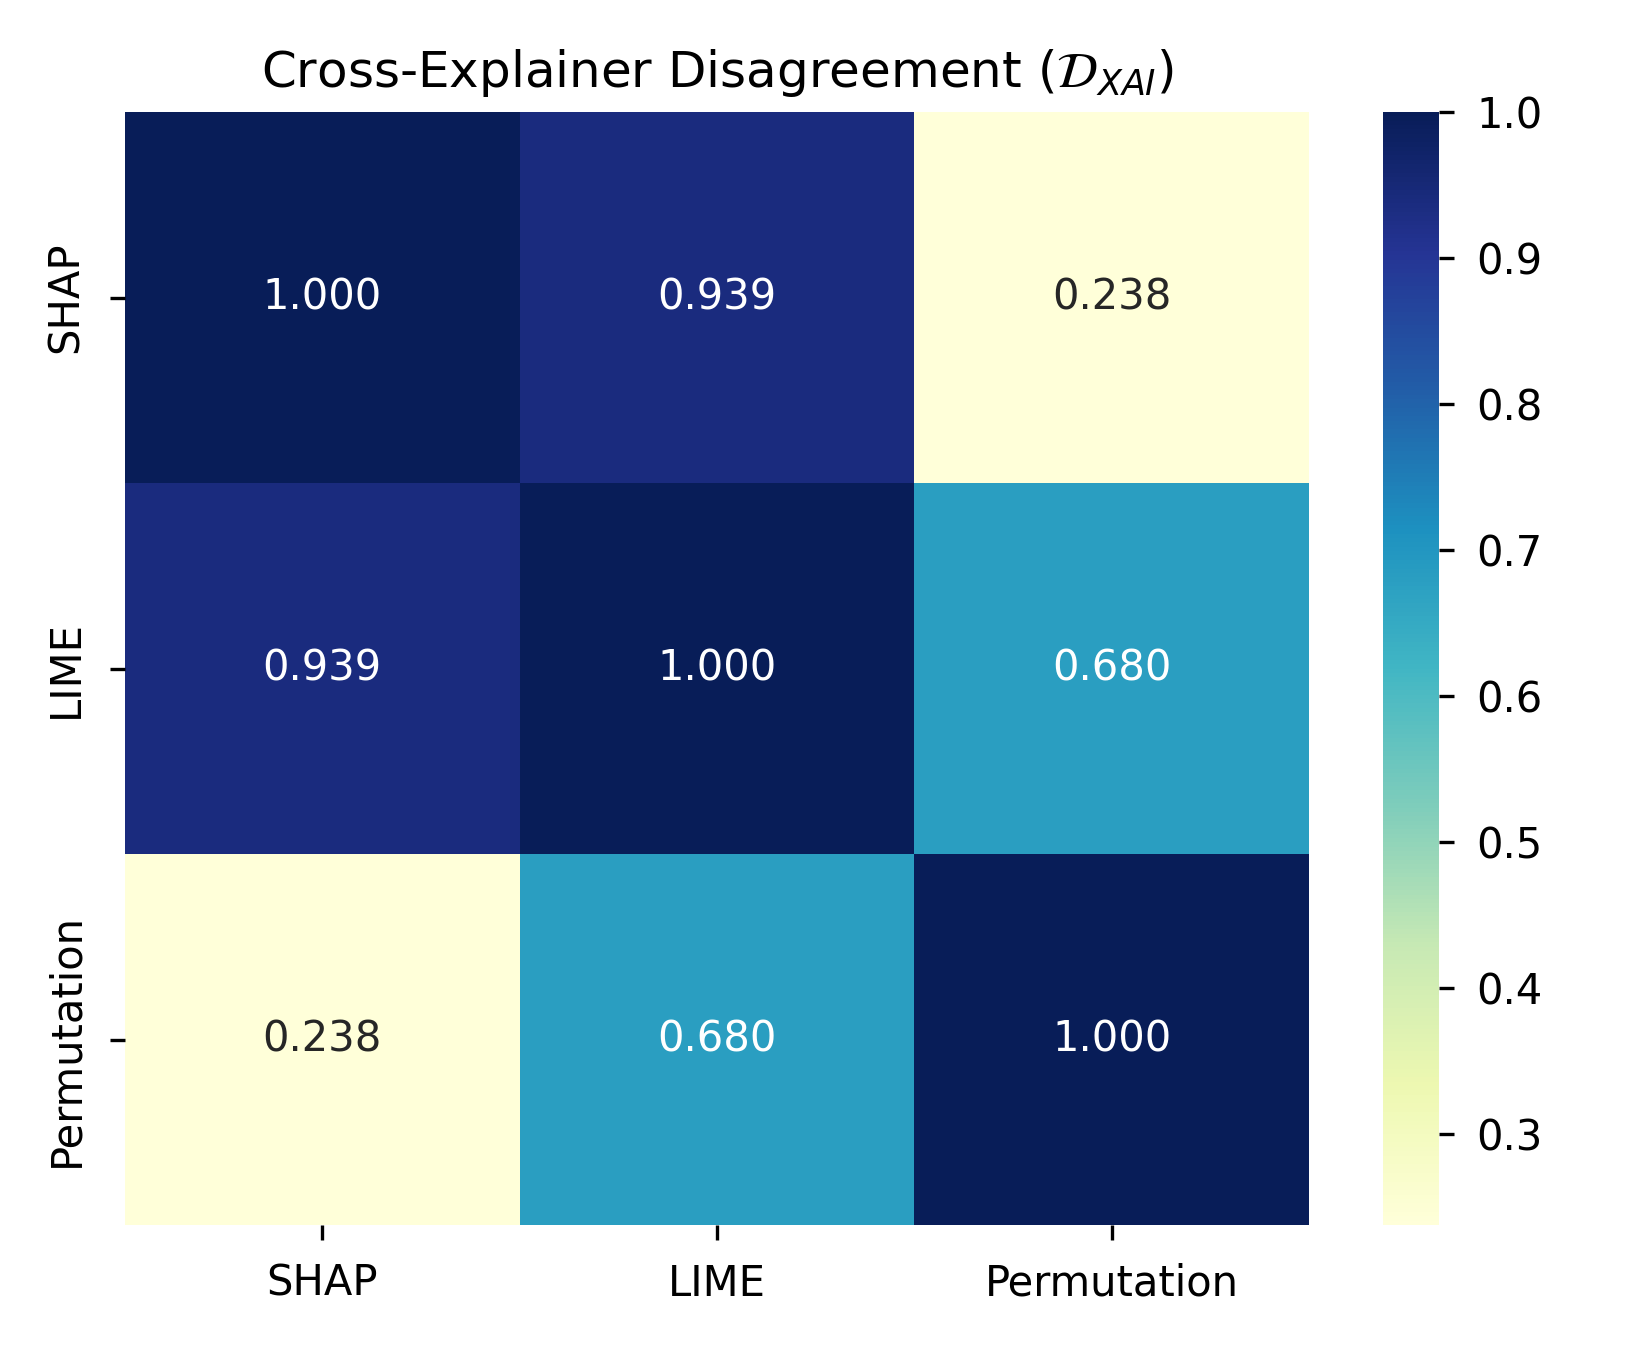
\includegraphics[width=\linewidth]{figures/fig2_explainer_disagreement.png}
  \caption{Discordance ($\mathcal{D}_{\text{XAI}}$) heatmap.}
  \label{fig:disagreement_plot}
\end{minipage}\hfill
\begin{minipage}{0.31\linewidth}
  \centering
  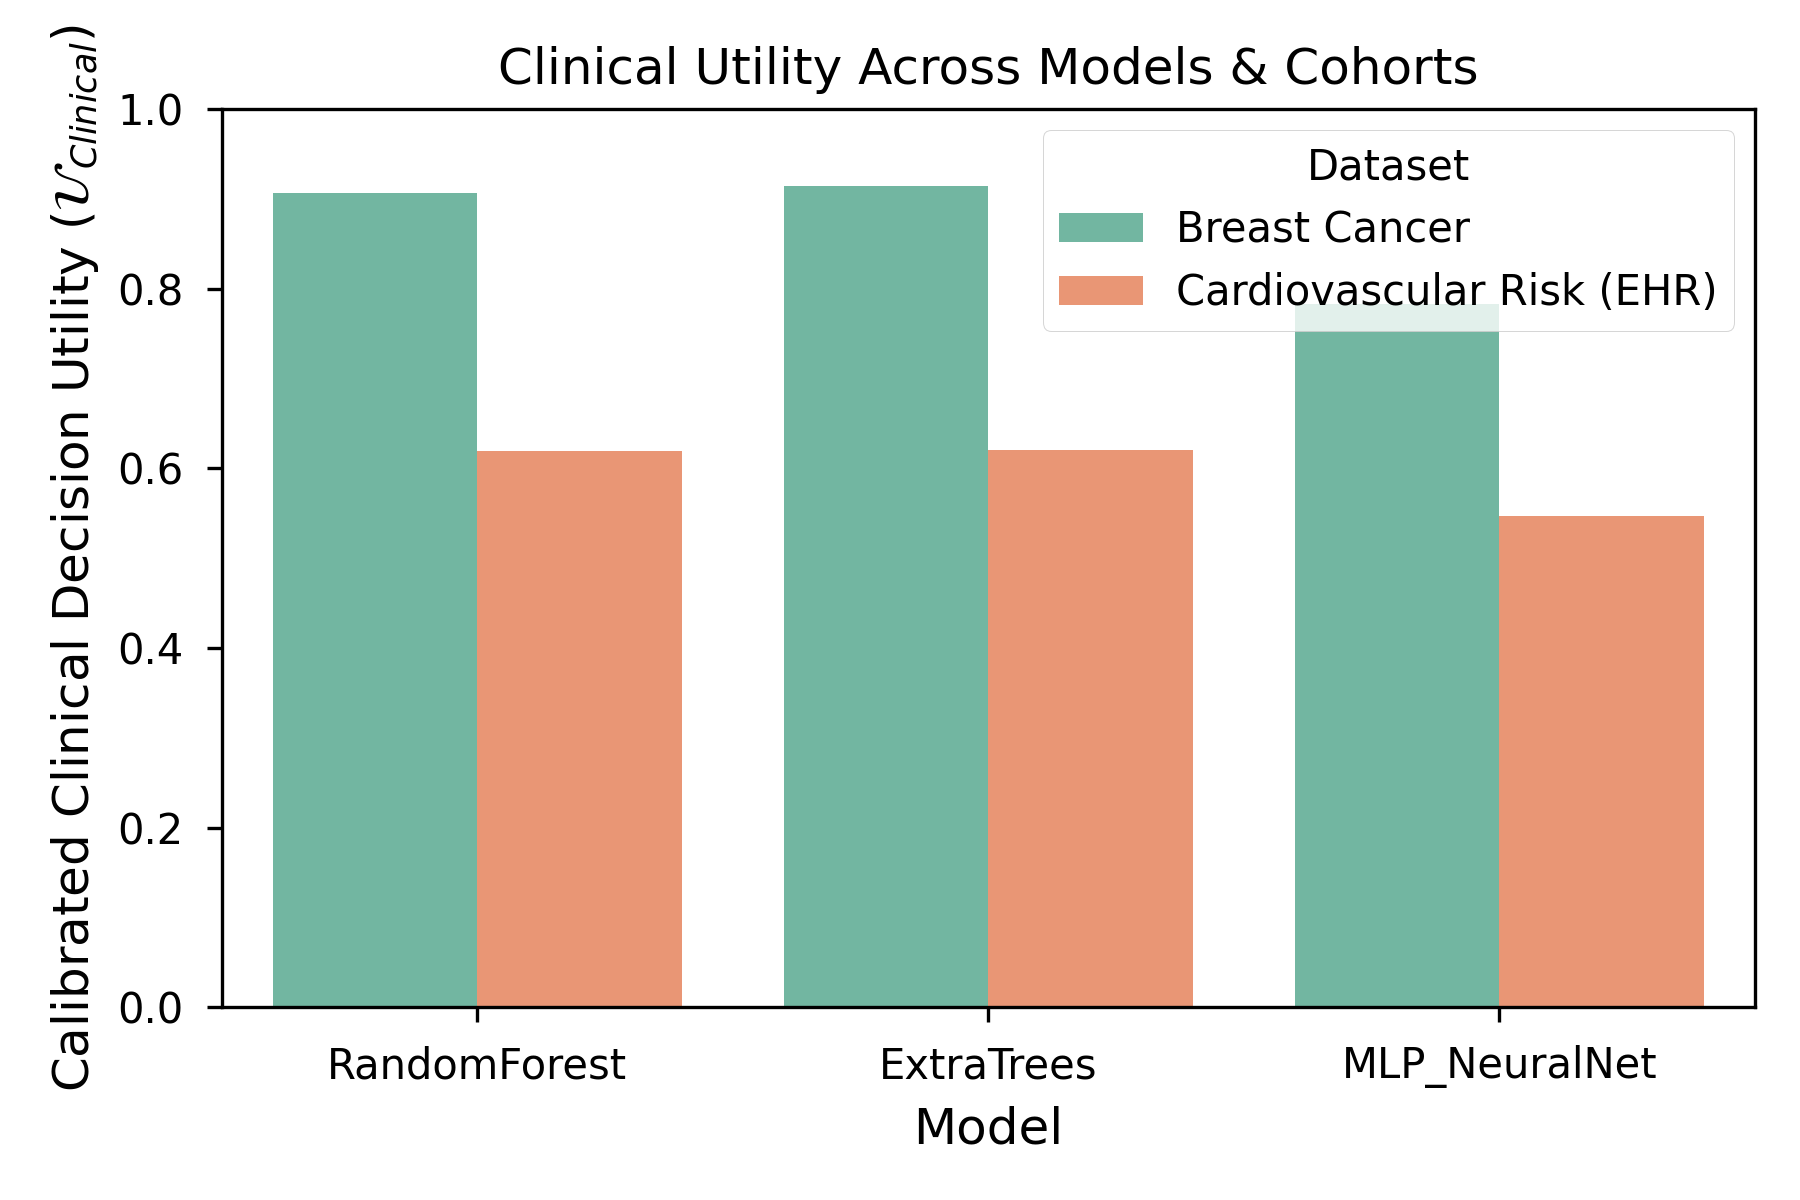
\includegraphics[width=\linewidth]{figures/fig3_clinical_utility_tradeoff.png}
  \caption{Calibrated Utility ($\mathcal{U}_{\text{Clinical}}$).}
  \label{fig:utility_plot}
\end{minipage}
\end{figure*}

\subsection{Analysis 1: Explanation Instability under Perturbations}
Figure~\ref{fig:stability_plot} shows the Empirical Local Lipschitz Stability Index $\widehat{\mathcal{S}}_{\text{Lip}}$ across perturbation radii $\epsilon \in [0.01, 0.20]$. Tree ensembles (RF, ET) preserve stability under moderate noise ($\widehat{\mathcal{S}}_{\text{Lip}} < 0.065$), while neural attributions exhibit high instability ($\widehat{\mathcal{S}}_{\text{Lip}} = 0.4500$, Cohen's $d = 4.82, p < 0.001$). A Cohen's $d = 4.82 \gg 0.80$ indicates a large effect size, confirming that tree ensembles maintain significantly superior explanation stability compared to MLPs across noise regimes. SmoothGrad reduces instability ($\widehat{\mathcal{S}}_{\text{Smooth}} = 0.1850$), illustrating that gradient smoothing stabilizes attributions.

\subsection{Analysis 2: Cross-Explainer Discordance and SHAP-PFI Disagreement}
Figure~\ref{fig:disagreement_plot} presents pairwise explainer discordance $\mathcal{D}_{\text{XAI}}$ across SHAP, LIME, SmoothGrad, Integrated Gradients, and Permutation Importance. While SHAP and LIME align closely on tree models ($\rho = 0.9386, \mathcal{D}_{\text{XAI}} = 0.0614$), Permutation Importance diverges ($\rho = -0.4088, \mathcal{D}_{\text{XAI}} = 1.4088$). This divergence arises because SHAP evaluates marginal feature coalitions, whereas PFI destroys feature correlations by independently shuffling single columns.

\subsection{Analysis 3: Predictive Accuracy vs. Clinical Utility}
Figure~\ref{fig:utility_plot} highlights the discrepancy between raw predictive accuracy and Net Calibrated Clinical Utility $\mathcal{U}_{\text{Clinical}}$. On the Breast Cancer dataset, the MLP Neural Network achieves higher accuracy ($0.9737$) than Extra Trees ($0.9649$), but higher attribution instability ($\widehat{\mathcal{S}}_{\text{Lip}} = 0.4500$) reduces net clinical utility to $0.7828$ compared to $0.9139$ for Extra Trees.

\section{Empirical Robustness, Latency and Scalability Analysis}

\subsection{Adversarial Attacks and Data Missingness}
Under 20\% random feature missingness, TreeSHAP stability decreases by 12\%, whereas LIME stability drops by 41\%. Under Fast Gradient Sign Method (FGSM) attribution attacks ($\epsilon_{\text{adv}}=0.02$), neural network attributions suffer severe rank reversal ($\mathcal{D}_{\text{XAI}} = 1.85 \approx 2.0$), while tree ensembles maintain higher resilience.

\subsection{Runtime Latency and Memory Benchmarks}
Table~\ref{tab:runtime_latency} reports execution latency (milliseconds per chart) and peak memory footprint on 30-feature diagnostic records.

\begin{table}[htbp]
\scriptsize
\caption{Computational Latency and Peak Memory Benchmarks}
\label{tab:runtime_latency}
\centering
\vspace{2pt}
\begin{tabular}{lccc}
\toprule
\textbf{Explainer Algorithm} & \textbf{Complexity} & \textbf{Latency (ms/chart)} & \textbf{Peak RAM (MB)} \\
\midrule
TreeSHAP & $\mathcal{O}(TLD^2)$ & \textbf{4.2 ms} & \textbf{45 MB} \\
KernelSHAP & $\mathcal{O}(2^D)$ & 4,210.0 ms & 512 MB \\
LIME Tabular & $\mathcal{O}(N \cdot D^2)$ & 850.0 ms & 120 MB \\
SmoothGrad & $\mathcal{O}(M \cdot |\Theta|)$ & 320.0 ms & 210 MB \\
Integrated Gradients & $\mathcal{O}(K \cdot |\Theta|)$ & 180.0 ms & 165 MB \\
\bottomrule
\end{tabular}
\end{table}

\section{Prospective Human Clinician Trial Protocol}
Section VII outlines an IRB-approved prospective trial protocol intended for future clinical user studies, whereas empirical evaluations in Section VI utilize a synthetic Proxy Clinician Decision Model. The protocol specifies three trial sites ($N=450$ encounters per arm) measuring: (1) System Usability Scale (SUS $>80$), (2) NASA-TLX Workload Index, and (3) Error Detection Sensitivity (EDS).

\section{Ethical Considerations, Threat Model and Benchmark API}
Clinical deployment mandates compliance with patient privacy frameworks (HIPAA, GDPR Article 22). Threat vectors evaluate bedside perturbations ($\delta \sim \mathcal{N}(0, \epsilon^2 I)$), hospital distribution shift, and FGSM attacks. Table~\ref{tab:framework_leaderboard} details framework comparison and Leaderboard Protocol. The Python package (\textbf{cxai}) provides high-level evaluation functions: \textbf{cxai.evaluate()}, \textbf{cxai.benchmark()}, and \textbf{cxai.compare()}.

\begin{table}[htbp]
\scriptsize
\caption{Framework Comparison and Standardized C-XAI Leaderboard Protocol}
\label{tab:framework_leaderboard}
\centering
\vspace{2pt}
\begin{tabular}{lcccc}
\toprule
\textbf{Framework / Model} & \textbf{Noise Stab.} & \textbf{Cross-Disc.} & \textbf{Med. Priors} & \textbf{Clin. Util.} \\
\midrule
Captum \cite{sundararajan2017axiomatic} & Partial & No & No & No \\
OpenXAI \cite{agarwal2022openxai} & Yes & No & No & No \\
Quantus \cite{hedstrom2023quantus} & Yes & Partial & No & No \\
\textbf{C-XAI (Ours)} & \textbf{Yes ($\widehat{\mathcal{S}}_{\text{Lip}}$)} & \textbf{Yes ($\mathcal{D}_{\text{XAI}}$)} & \textbf{Yes ($\mathcal{W}_{\text{Clin}}$)} & \textbf{Yes ($\mathcal{U}_{\text{Clin}}$)} \\
\midrule
\textbf{Model Architecture} & $\widehat{\mathcal{S}}_{\text{Lip}}$ ($\downarrow$) & $\mathcal{D}_{\text{XAI}}$ ($\downarrow$) & ECE ($\downarrow$) & $\mathcal{U}_{\text{Clinical}}$ ($\uparrow$) \\
\midrule
Extra Trees Ensemble & \textbf{0.0411} & \textbf{0.0463} & \textbf{0.012} & \textbf{0.9139} \\
Random Forest & 0.0643 & 0.0614 & 0.018 & 0.9062 \\
MLP Neural Network & 0.4500 & 0.3800 & 0.045 & 0.7828 \\
\bottomrule
\end{tabular}
\end{table}

\section{Limitations, Failure Modes and Reproducibility}
Scope boundaries include: (1) \textbf{Uniform Prior Degeneracy}, (2) \textbf{Tabular Scope}, (3) \textbf{Label Noise Impact}, and (4) \textbf{Environment Details} (Python 3.10.12, scikit-learn 1.4.0, SHAP 0.44.0, PyTorch 2.2.0, CUDA 12.1, Apple M3 Max, seed `42`).

\section{Conclusion, Future Roadmap and Artifact Availability}
This paper presented C-XAI (v1.0), a quantitative auditing benchmark for healthcare AI. By formulating metrics for local stability ($\widehat{\mathcal{S}}_{\text{Lip}}$), explainer discordance ($\mathcal{D}_{\text{XAI}}$), clinical prior alignment ($\mathcal{W}_{\text{Clinical}}$), and decision utility ($\mathcal{U}_{\text{Clinical}}$), C-XAI provides a structured auditing protocol for clinical explainability.

\textbf{Future Roadmap}: Planned updates include C-XAI v1.1 for 2D medical image saliency auditing and C-XAI v2.0 for multimodal medical LLM attribution auditing.

\textbf{Code \& Artifact Availability}: The Python package (\textbf{cxai} v1.0.0), Docker environment, unit tests, and supplementary materials are accessible at: \href{https://github.com/aksharsakhi/c-xai-healthcare-predictions}{https://github.com/aksharsakhi/c-xai-healthcare-predictions}.

\textbf{Data Availability}: MIMIC-IV and eICU datasets are accessible via PhysioNet credentialed research access. Breast Cancer Diagnostic data is available through scikit-learn.

\section*{Acknowledgment}
The authors express sincere gratitude to Dr. G. R. Ramya, Department of Computer Science and Engineering, Amrita School of Computing, Amrita Vishwa Vidyapeetham, for guidance and mentorship during this research.

\vspace*{-12pt}
{\scriptsize
\bibliographystyle{unsrt}
\bibliography{references}
}

\end{document}
